\begin{frame}{Conditions}
    \bigskip
    \setlength{\arrayrulewidth}{0.2mm}
    \setlength{\tabcolsep}{08pt} % padding on sides
    \renewcommand{\arraystretch}{1.2} % height

    \centering
    \small
    \begin{tabular}{ |p{4cm}|p{1.5cm}|p{1.5cm}|p{1.5cm}| }
        \hline
        Gas flow (constant: $50$ mL/min, $0.3$ bar) & RT & \textcolor{Important}{300°C} & \textcolor{Important}{400°C} \\
        \hline
        Argon (inert gas) & \multicolumn{3}{l|}{Catalyst state without reactants (unactive)}\\ \hline
        1 \ammonia & \multicolumn{3}{l|}{NH3 introduction influence}\\ 
        \hline
        1 \ammonia + 0.5 \dioxygen & \multicolumn{3}{c|}{}\\
        1 \ammonia + 1 \dioxygen & \multicolumn{3}{c|}{\multirow{-2}{*}{Influence of \ammonia / \dioxygen ratio as a function}}\\
        1 \ammonia + 2 \dioxygen & \multicolumn{3}{c|}{\multirow{-2}{*}{of the temperature and vice-versa}}\\
        1 \ammonia + 8 \dioxygen & \multicolumn{3}{c|}{} \\ 
        \hline
    \end{tabular}

    \pause
    \begin{figure}
        \centering
        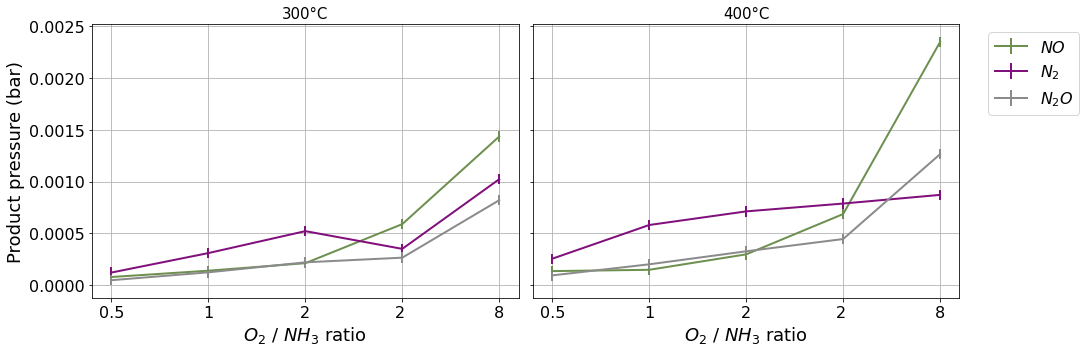
\includegraphics[width=0.9\textwidth]{Figures/sxrd_data/rga/product_comparison.png}
        \label{fig:product_pressure}
        \caption{Product pressure evolution with temperature and input gas}
    \end{figure}
    
\end{frame}